\section{Binomická věta}

Kombinační čísla mají kromě kombinatorických úloh využití i v klasické aritmetice. Ať už se to zdá, nebo ne, tyto dva možná zdánlivě rozdílné světy si nejsou až tak vzdálené. V této sekci se proto podíváme na větu, která nám trochu více zobecní koncept roznásobování dvojčlenů.\par
Podívejme se nejdříve na ty nejjednodušší případy:
\begin{align*}
    (x+y)^0&=1,\\
    (x+y)^1&=x+y,\\
    (x+y)^2&=x^2+2xy+y^2,\\
    (x+y)^3&=x^3+3x^2y+3xy^2+y^3,\\
    (x+y)^4&=x^4+4x^3y+6x^2y^2+4xy^3+y^4,\\
    &\vdots
\end{align*}
Čeho bychom si mohli na poprvé možná všimnout je faktu, že koeficienty u jednotlivých členů jsou symetrické. To je asi nejlépe vidět u roznásobení čtvrté mocniny dvojčlenu $x+y$. Proč tomu ale tak je? Vzpomeňme si na větu \ref{thm:symetrie_kombinacnich_cisel}, díky které jsme se dozvěděli, že kombinační čísla jsou "symetrická", tzn. $\binom{n}{k}=\binom{n}{n-k}$. Další pozorování bychom z tohoto zápisu učili nejspíše stěží (avšak klobouček dolů všem, kteří to již vidí :-)). Zkusme se zaměřit nyní čistě na dané koeficienty. Počet členů je vždy totiž lichý, což nám umožňuje zapsat si jejich koeficienty ve schématu níže.
\begin{figure}[H]
    \centering
    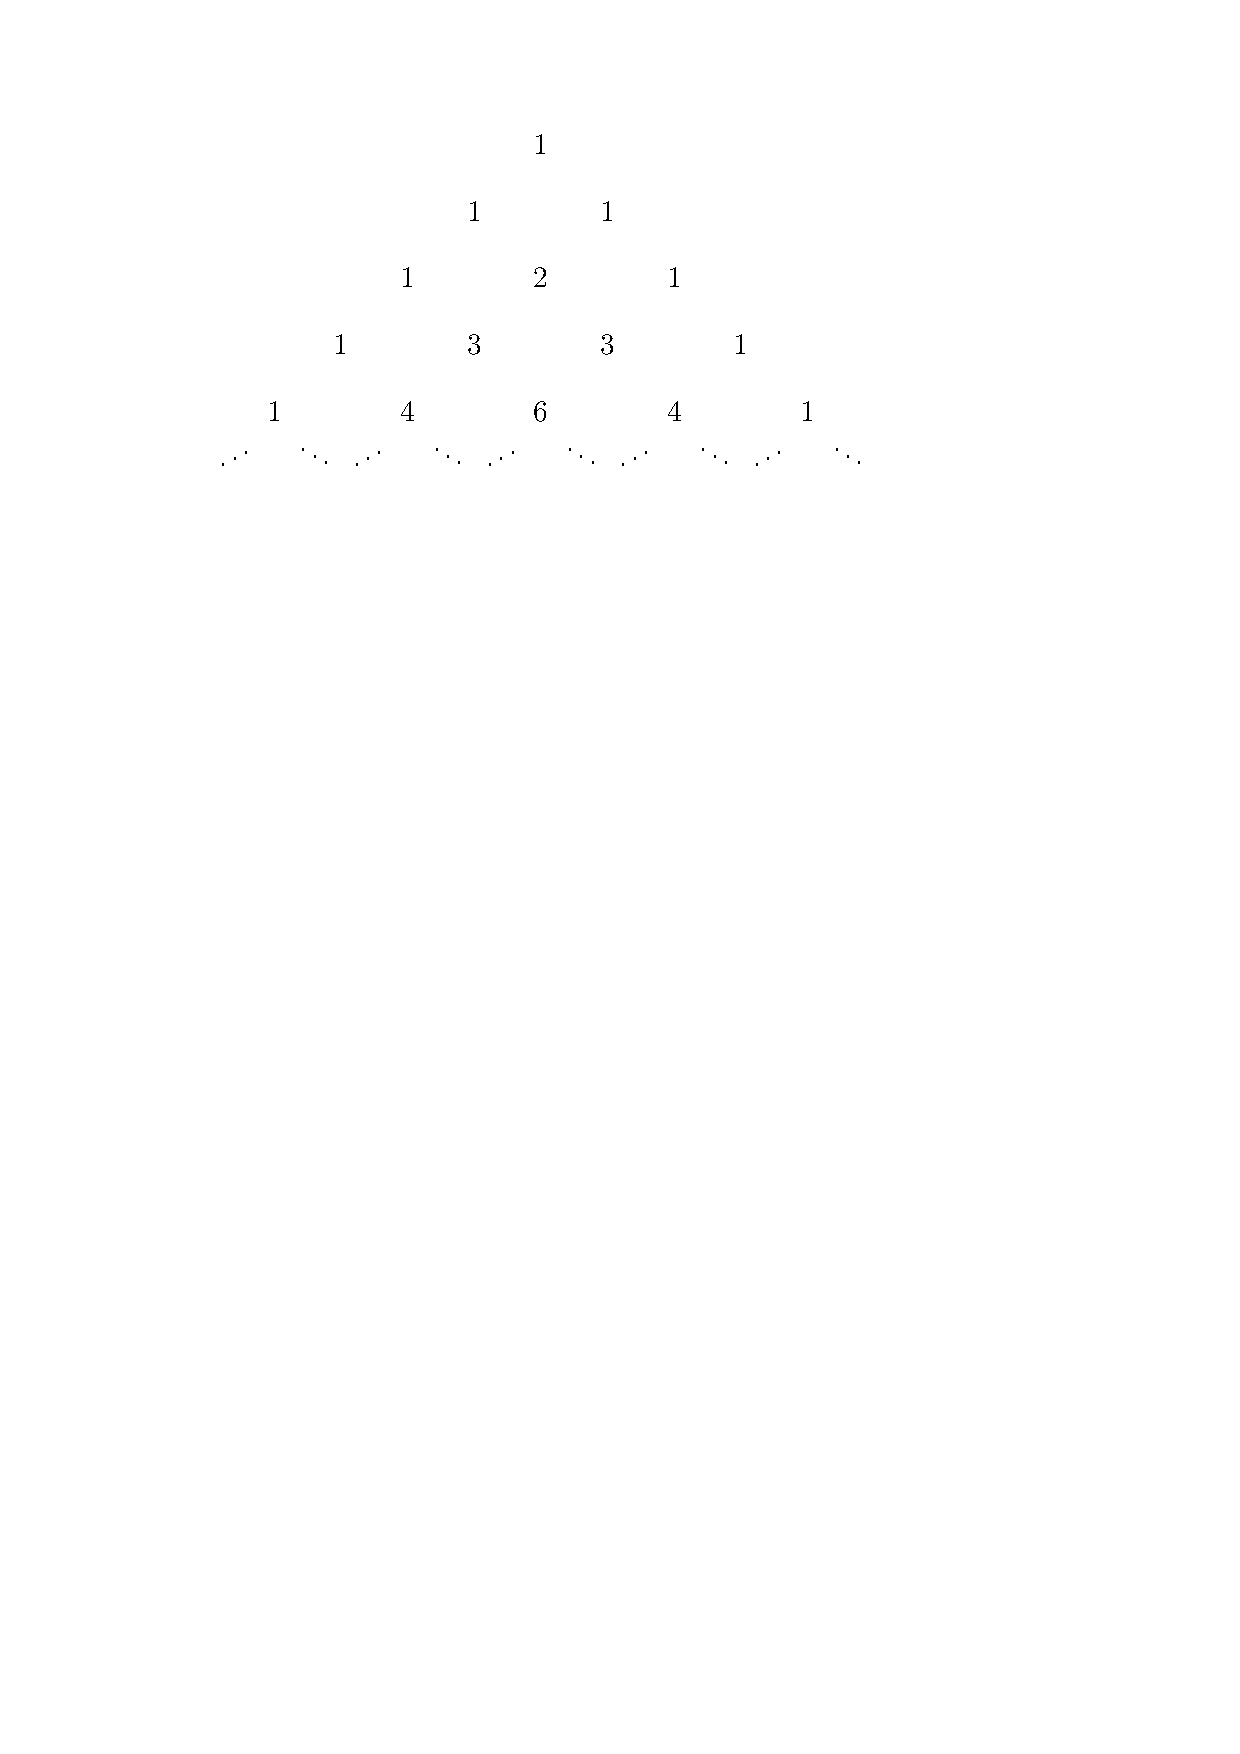
\includegraphics[scale=\normalipe]{ch03_pascaluv_trojuhelnik.pdf}
    \caption{Schéma koeficientů ve tvaru pyramidy.}
    \label{fig:pascaluv_trojuhelnik}
\end{figure}
Toto schéma se nazývá \textbf{Pascalův trojúhelník}. Pokud se podíváme blíže, lze si všimnout, jak vznikají jeho řádky. Na kraji vždy pevně stojí číslo 1 a další koeficienty vzniknou součtem koeficientů nad ním.
\begin{figure}[H]
    \centering
    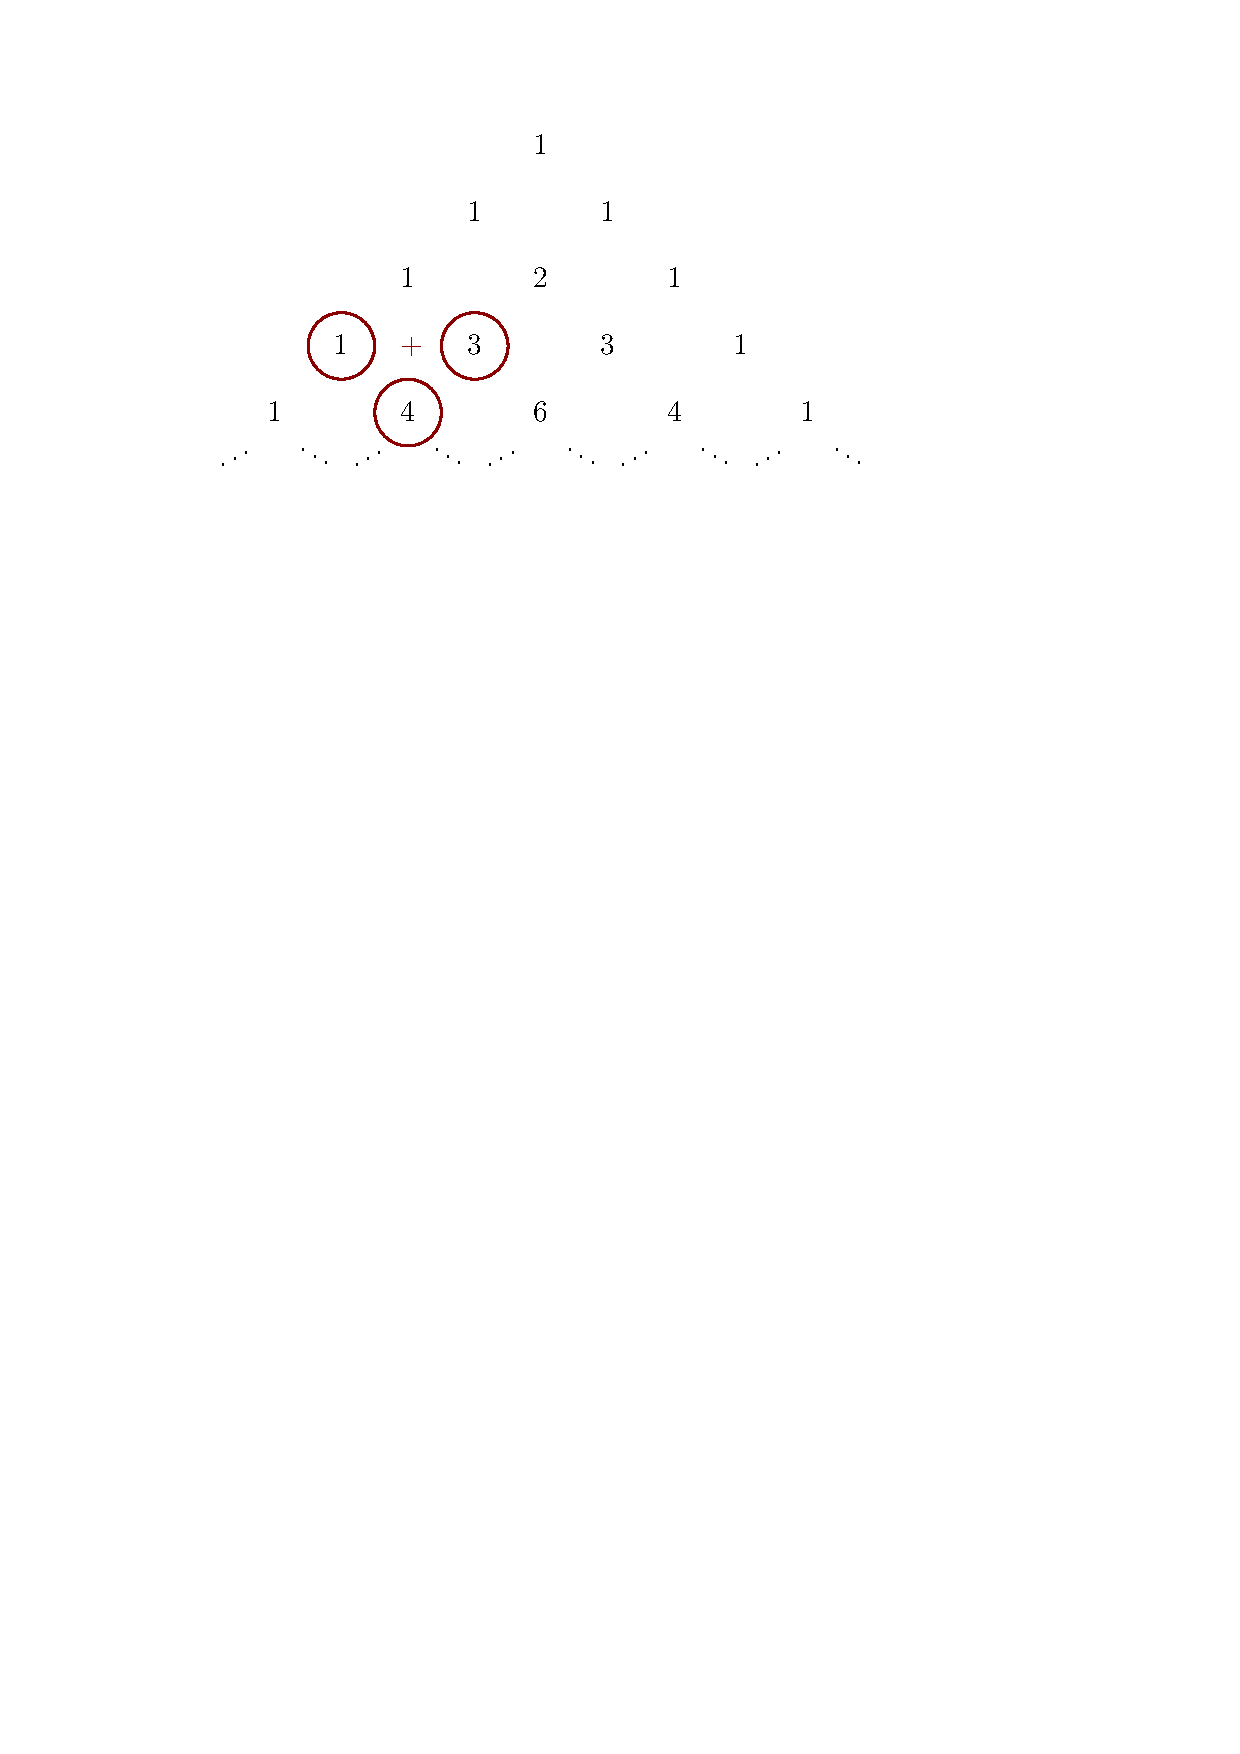
\includegraphics[scale=\normalipe]{ch03_pascaluv_trojuhelnik_soucet.pdf}
    \caption{Generování Pascalova trojúhelníku součtem členů.}
    \label{fig:pascaluv_trojuhelnik_soucet}
\end{figure}
Pokud se nyní vrátíme opět ke kombinačním číslům, jistě si vzpomeneme, že jsme zde měli větu \ref{thm:soucet_kombinacnich_cisel}, která dávala do souvislosti kombinační čísla a jejich součet. Z toho by nás tak mohlo napadnout, že jednotlivá čísla v Pascalově trojúhelníku by tak mohla odpovídat jistým kombinačním číslům. Je tomu skutečně tak.
\begin{figure}[H]
    \centering
    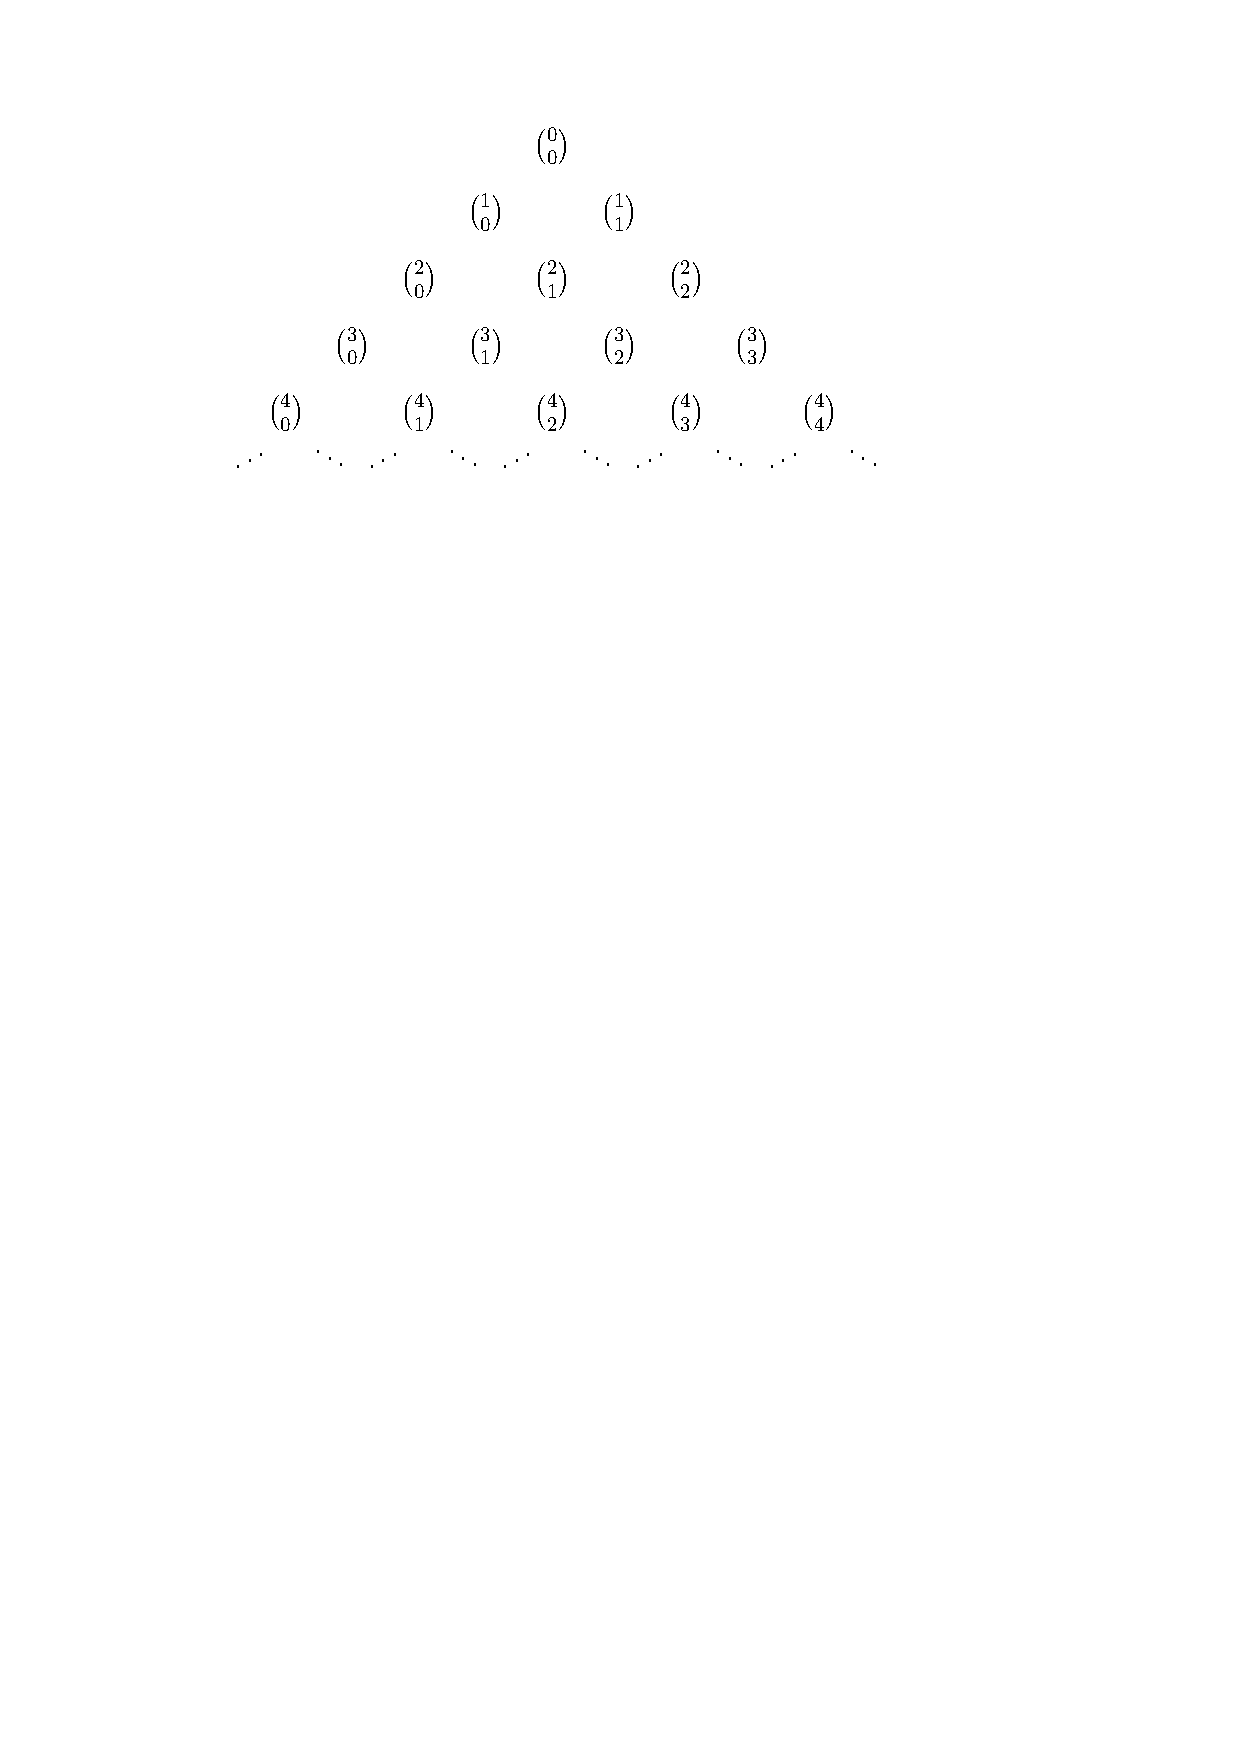
\includegraphics[scale=\normalipe]{ch03_pascaluv_trojuhelnik_kombinacni_cisla.pdf}
    \caption{Pascalův trojúhelník pomocí kombinačních čísel.}
    \label{fig:pascaluv_trojuhelnik_kombinacni_cisla}
\end{figure}
Sami se můžete přesvědčit, že jednotlivá kombinační čísla odpovídají daným koeficientům. Navíc zde lze i vidět i jejich další vlastnosti v uplatnění, konkrétně věty \ref{thm:symetrie_kombinacnich_cisel} (stačí se podívat na $k$-tý člen a příslušném $(n-k)$-tý člen, kde $n$ zde představuje číslo řádku od nuly, neboť odpovídá mocnině daném dvojčlenu) a \ref{thm:soucet_kombinacnich_cisel} (koeficient různý od jedničky na kraji je součtem koeficientů nad ním).\par

Vraťme se nyní k roznásobování dvojčlenů. Z Pascalova trojúhelníku lze tak vidět, že koeficienty v rozvoji $(x+y)^n$ by mohly být po řadě čísla
\[\binom{n}{0},\,\binom{n}{1},\,\binom{n}{2},\,\cdots,\,\binom{n}{n}.\]
Jak lze ukázat, platí totiž následující věta.
\begin{theorem}[Binomická]
    Pro libovolná $x,\,y\in\C$ a $n\in\N$ platí
    \[(x+y)^n=\sum_{k=0}^{n}\binom{n}{k}x^{n-k}y^k,\]
    neboli
    \[(x+y)^n=\binom{n}{0}x^ny^0+\binom{n}{1}x^{n-1}y^1+\binom{n}{2}x^{n-2}y^2+\cdots+\binom{n}{n}x^0y^n.\]
\end{theorem}